\MTtitle{Aprendizaje automático}


%------------------------------------Inteligencia Artificial-------------------------------%
\section{Inteligencia Artificial}

Son muchas las definiciones que se encuentran de la inteligencia artificial o IA, en sus inicios se propone como las  actividades asociadas al pensamiento humano, tareas como, toma de decisiones, resolución de problemas y aprendizaje \citep{CT19}. Con el paso de los años se ha acuñado una definición mas completa: ``la Inteligencia Artificial es una ciencia orientada al diseño y construcción de máquinas que implementen tareas propias de humanos dotados de inteligencia'' \citep{CT1}.\\


Esta ciencia contribuye en el desarrollo de diversos campos de investigación como, Redes neuronales, Computación evolutiva, Algoritmos genéticos, Programación Genética, Teoría del caos. Además tiene un campo amplio de aplicaciones en la sociedad \citep{CT20}, a continuación se muestran algunos ejemplos:

\begin{itemize}

	\item \textbf{Vehículos robóticos}: Un auto robótico sin conductor llamado STANLEY aceleró a través del terreno de Mojave a 22 mph (\textit{miles per hour}, por sus siglas en ingles), terminando el curso de 132 millas primero para ganar el Gran Desafío DARPA 2005.

	\item \textbf{Reconocimiento de voz}: Un viajero que llama a \textit{United Airlines} para reservar un vuelo puede tener la conversación completa guiada por un sistema automático de reconocimiento de voz y gestión de diálogos.

	\item \textbf{Planificación y programación autónoma}: A cien millones de millas de la Tierra, el programa \textit{Remote Agent} de la NASA se convirtió en el primer programa autónomo de planificación a bordo para controlar la programación de operaciones de una nave espacial.

	\item \textbf{Robótica}: \textit{iRobot Corporation} ha vendido más de dos millones de aspiradoras robóticas \textit{Roomba} para uso doméstico.

	\item \textbf{Máquina traductora}: Un programa de computadora  traduce automáticamente del árabe al inglés.

\end{itemize} 
 

%----------------------Procesamiento de lenguaje natural-------------------------------------%

\section[Procesamiento de LN]{Procesamiento de lenguaje natural}

El procesamiento de lenguaje natural es una disciplina de la Inteligencia Artificial que se ocupa de la formulación e 
investigación de mecanismos computacionales para la comunicación entre personas y maquinas mediante el uso de Lenguajes 
Naturales.\\

Este campo incluye diferentes técnicas para interpretar el lenguaje humano, que van desde los métodos 
estadísticos y del aprendizaje basado en máquina hasta los enfoques basados en reglas y algorítmicos. Necesitamos una amplia variedad 
de métodos porque los datos basados en texto y en voz varían ampliamente, al igual que las aplicaciones prácticas. 


%------------------------------------Apredizje automático-------------------------------%
\section{Aprendizaje Automático}

EL Aprendizaje Automático es una rama de la Inteligencia Artificial; permite desarrollar algoritmos que tienen la capacidad de extrapolar (\textit{i.e} predecir) los cambios que se acontecen en una tarea específica \citep{CT2}.\\

EL campo utiliza una variedad de algoritmos que aprenden iterativamente de un conjunto de
datos para describir y predecir resultados. A medida en la cual los algoritmos de 
entrenamiento obtienen datos es posible obtener modelos más precisos. Existen cuatro clasificaciones en los métodos \citep{CT21}:

\begin{itemize}

	\item \textbf{Aprendizaje supervisado}: Se proporciona un conjunto de datos de entrenamiento con las respuestas correctas y, con base a este conjunto de 
	entrenamiento, el algoritmo se generaliza para responder correctamente a todas 
	las entradas posibles.

	\item \textbf{Aprendizaje no supervisado}: No se proporcionan datos de entrenamiento, el algoritmo intenta identificar similitudes entre las entradas para clasificar en conjuntos. El enfoque estadístico del aprendizaje no 
	supervisado se conoce como estimación de densidad.

	\item \textbf{Aprendizaje reforzado}: Está en algún lugar entre el aprendizaje supervisado y no supervisado. Se indica al algoritmo cuando la respuesta es incorrecta, sin embargo no se informa
	cómo corregirlo. Tiene que explorar y probar diferentes posibilidades hasta que resuelva 
	cómo obtener la respuesta correcta.

	\item \textbf{Aprendizaje evolutivo}: La evolución biológica puede verse como un proceso de aprendizaje: los organismos biológicos se adaptan para mejorar sus tasas de supervivencia 
	y la posibilidad de tener descendientes en su entorno. Este comportamiento es modelado, 
	usando un modelo física, el cual corresponde a una puntuación en la 
	solución actual.

\end{itemize}

Cabe mencionar que el método implementado en este trabajo es el aprendizaje supervisado, mas a delante se da una explicación detalla.\\

El aprendizaje automático se puede aplicar a una amplia gama de problemas comerciales, desde la detección de fraudes hasta la orientación al cliente y la recomendación de productos, al monitoreo industrial en tiempo real, el análisis de sentimientos y el diagnóstico médico. Puede asumir problemas que no pueden administrarse manualmente debido a la gran cantidad de datos que deben procesarse \citep{CT22}. Cuando se aplica a grandes conjuntos de datos, a veces puede encontrar relaciones tan sutiles que ninguna cantidad de escrutinio manual las descubriría nunca. Y cuando muchas de estas relaciones ``débiles'' se combinan, se convierten en predictores fuertes.





%------------------------------------Apredizje automático para texto------------------------%

\section[AA Para texto]{Aprendizaje automático para texto}

La extracción de información útil con varios tipos de algoritmos estadísticos es denominado \textbf{Extracción de datos} (\textit{text mining}), \textbf{Analítica de texto} (\textit{text analytics}) o \textbf{Aprendizaje automático para texto} (\textit{Machine learning for text}) \citep{CD1}. En los últimos años este campo ha incrementado por el desarrollo de la web, redes sociales, correos electrónicos, bibliotecas virtuales. Algunas de las aplicaciones son las siguientes:

\begin{itemize}

	\item Etiquetar la web, permite al usuario encontrar paginas de interés

	\item Los proveedores de correos, utilizan la información almacenada para mostrar publicidad de interés al usuario

	\item Algunas páginas ordenan su contenido de acuerdo a su importancia

	\item El análisis de las opiniones es un campo de importancia así como el análisis de sentimientos		

\end{itemize}

El orden de las palabras en un texto brindan un significado semántico el cual no puede ser inferido  solo con la frecuencia de las palabras. Sin embargo, se pueden hacer varias predicciones sin contemplar la semántica. Existen dos tipos de representaciones que son populares:

\begin{itemize}
	
	\item \textbf{Texto como una bolsa de palabras}: Es la representación mas común. No se contempla el orden de las palabras el proceso. El conjunto de palabras en el documento se convierten en \textit{Sparse multidimentional reprentation}, el cual corresponde a la dimensión en esta representación. Se utiliza para la clasificación, sistemas de recomendación.

	\item \textbf{Texto como un conjunto de secuencias}: En esta representación se extraen sentencias, el orden de las palabras si importa. La unidad son sentencia o párrafos. Es utilizado en aplicaciones que necesitan un fuerte uzo de la semántica, esta área se acerca mucho al modelado de lenguaje y procesamiento del lenguaje natural.

\end{itemize}


%----------------------------------Representación del texto--------------------------%
\subsection[Representación del T]{Representación del texto}
Los métodos de Aprendizaje Automático requieren que la información de la cual aprenderán esté representada en un
formato que facilite su procesamiento. Generalmente esta representación es mediante vectores de valores numéricos. 
Cuando se requiere utilizar estos métodos con información en forma de texto, dicha
información debe ser transformada para generar una representación más adecuada. 


%------------------------------------Pre-procesamiento------------------------%

\subsection[Pre-procesamiento]{Pre-procesamiento}

El Pre-procesamiento es necesario para convertir el formato no estructurado en un formato estructurado \citep{CD1}.
A menudo el texto contiene información extraña como etiquetas, \textit{anchor text}\footnote{Es el texto mostrado en los enlaces o hipervínculos, \textbf{Texto de anclaje} en español.}, y otras características. En muchos casos las palabras son variaciones de otros (sinónimos) por el tipo de redacción, el contexto, para eliminar redundancia. Algunas palabras simplemente tienen faltas de ortografía. El proceso de convertir una secuencia de caracteres en una secuencia de palabras (tokens), es llamado ``Tokenización''.

%---------------------------------Extracción de texto-------------------------%

\subsection{Extracción de texto}

Cuando se recupera  información de la web, se tiene que limpiar el texto ya que contiene etiquetas definidas por el hipertexto. Se debe buscar los bloques que brinden información útil para el ambito de estudio, algunas secciones contienen publicidad o información no relacionada a los datos de interes. Para esto se tiene que realizar un análisis para discriminar la información útil \citep{CD1}.


	%\item \textbf{Remover stop-words}: Son pronombres y preposiciones que deben ser removidas para mejorar la compresión del texto.

	%\item  \textbf{Stemming, case-folding, punctuation}: Las palabras que derivan de la misma raíz como hundimiento, se hundió, se reducen a hundir. Una palabra puede tener diferentes significados dependiendo el contexto como la palabra \'Rosa\' puede hacer referencia a una flor o el nombre de una persona, por lo tanto se requiero la heurística del lenguaje específico para poder tomar una decisión en como debe ser interpretada. Los signos de puntuación como el guión medio deben ser tratados con mucho cuidado para realizar una buena tokenización.

%---------------------------------------------Corpus-----------------------------------------%

\subsection{Corpus}

Se le llama corpus a la recopilación de un conjunto de textos, de materiales escritos y/o hablados, 
agrupados bajo un conjunto de criterios mínimos, para realizar ciertos análisis lingüísticos.


%-----------------------------------------Tokenización-------------------------------------%

\subsection{Tokenización}

Es el proceso que descompone los textos de una colección en sus unidades mínimas, las palabras
o términos propiamente dichos. A tales elementos se les denomina tokens que conforman una lista de
ítems que se utiliza para su análisis estadístico, ling{\"u}ístico, de almacenamiento y posteriormente de
recuperación de información. Los tokens a su vez pueden ser identificados mediante una codificación
ASCII o en su defecto hexadecimal, con el objeto de facilitar la identificación uno a uno cada caracter
que compone la palabra. De hecho, este proceso permite la identificación de cadenas de caracteres de
forma unívoca, de cara a posteriores tratamientos de depuración, eliminación de signos de puntiación
o la reducción morfológica \citep{CT12}.

Ejemplo  (\ref{tabla:sencilla}): Hoy es un gran día para salir.

\begin{table}[htbp]
	\begin{center}
	\begin{tabular}{|l|r|r|c|c|c|c|c|}
		\hline
		ID & 1 & 2 & 3 & 4 & 5 & 6 & 7 \\ 
		\hline
		Token & Hoy & es & un & gran & día & para & salir \\ \hline
		\hline
	\end{tabular}
	\caption{Ejemplo de tokenización}
	\label{tabla:sencilla}
	\end{center}
	
\end{table}

%-----------------------------------------Lematización-------------------------------------%

\subsection{Lematización}

Es el proceso lingüstico que, dada una palabra flexionada se encuentra su
lema. Una palabra flexionada es cuando esta en el plural, en femenino conjugada,
diminutivo o en superlativo. El lema es la palabra que esta en singular para
sustantivo, singular masculino para adjetivo e infinitivo para un verbo \citep{CT13}. Ejemplo:

	\begin{itemize}
		\item amigos, amiga, amiguitos-> Amigo
		\item soy, son, es->Ser
	\end{itemize}

Cabe mencionar que existen diversos grados de lematización

	\begin{itemize}
		\item Mórfólogica: Es la anterior mente explicada
		\item Sintáctica: Toma encuenta el contexto donde se encuentra la palabra

	\end{itemize}

Una opción para lematizar es \textit{Freeling} \citep{CT18}, este es un lematizador hecho por la
universidad de catalunia.

%------------------------------Frecuencia inversa del documento-------------------------------%

\subsection{Frecuencia inversa del documento}

Las palabras con poca frecuencia son mas discriminatorias que las de alta frecuencia. Por lo tanto se pondera la importancia de los documentos con base al calculo de la \textbf{frecuencia inversa del documento}(\textit{fid}) en la colección. Si $\psi_i$ es el número de documentos en el cual la palabra aparece, y $\psi$ es el número total de documentos, la \textit{fid} se calcula como $log(\frac{\psi}{\psi_i})$. La importancia de un documento se calcula multiplicando la \textbf{frecuencia de término} (\textit{ft}) en el documento por la \textit{fid}. Mientras la \textit{ft} brinda la cantidad de veces  que una palabra aparece en el documento la \textit{fid} especifica la importancia en la colección; Se define como \textbf{ft-fid} o \textit{tf-idf} (Por su sigla en ingles \textit{Term frequency – Inverse document frequency}) es la multiplicación de $ft$ por $idf$ \citep{CD1}.



%------------------------------------Aprendizaje Supervisado----------------------------------%

\section[A Supervisado]{Aprendizaje supervisado}

Los algoritmos de aprendizaje supervisado dependen de datos previamente etiquetado, es decir se necesita un corpus de datos, para llevar acabo el entrenamiento, así 
el algoritmo pueda comprender los datos y con ello determinar que etiqueta debe asignarse a los nuevos datos 
en función del patron y asociando los patrones a los nuevos datos sin etiquetar. Después de ello, la maquina recibe 
un nuevo conjunto de datos para que el algoritmo de aprendizaje supervisado analice los datos y produzca un resultado 
correcto de los datos etiquetados \citep{CT4}.\\


%------------------------------------Regresión logistica----------------------------------%

\subsection{Regresión logística}

La regresión logística es una técnica estadística multivariante que nos permite estimar la relación existente entre una variable dependiente 
no métrica (donde la variable es binaria o también conocida como dicotómica, es decir, solo va a dar como resultado dos alternativas posibles) 
y un conjunto de variables independientes métricas o no métricas \citep{CT6}. Es útil para modelar la probabilidad de un evento ocurriendo como 
función de otros factores. El análisis de regresión logística se enmarca en el conjunto de Modelos Lineales Generalizados que usa como función de 
enlace la función logit. Las probabilidades que describen el posible resultado de un único ensayo se modelan, como una función de variables explicativas, 
utilizando una función logística.\\

La regresión logística es usada extensamente en las ciencias médicas y sociales. Otros nombres para regresión logística usados en varias áreas de 
aplicación incluyen modelo logístico, modelo logit, y clasificador de máxima entropía.

%------------------------------------Naive bayes----------------------------------------%

\subsection{Naive bayes}

Naive Bayes es un conjunto de algoritmos de aprendizaje supervisado que se basan en la aplicación del teorema de Bayes con "Naive" 
(ingenuo) la cual es la supuesta de independencia condicional entre cada par de características dado el valor de la variable de clase. 

La clasificación Naive Bayes son aproximaciones probabilísticas, las cuales hacen especulaciones sobre como deben de ser 
generados los datos. Generalmente utilizan aprendizaje supervisado sobre el conjunto de entrenamiento para poder estimar los parámetros 
del modelo generativo, en tanto el conjunto de datos de entrada nuevos se realiza el teorema de Bayes, seleccionando la probable categoría 
que se ha generado \citep{CT7}.
\\
Todas las características extraídas que utilizan este clasificador son independientes entre sí. La ventaja de usar este clasificador es que 
funciona bien tanto con datos numéricos como con datos textuales y, además, es más fácil de implementar. La desventaja de este clasificador es 
que su rendimiento empeora cuando las características extraídas se correlacionan entre sí.

%----------------------------Maquina de soporte vectorial-------------------------------------%

\subsection{Maquina de soporte vectorial}

Las máquinas de soporte vectorial son sistemas de aprendizaje los
cuales se basan en el uso de un espacio de funciones lineales en un espacio de mayor dimensión inducido
por un kernel, en el que las hipótesis son entrenadas por un algoritmo\citep{CT8}.
Han sido implementadas en clasificación de imágenes, reconocimiento de caracteres, detección de
proteínas, clasificación de patrones, identificación de funciones,etc.
Pertenecen a la categoría de los clasificadores lineales, debido a que inducen separadores lineales
(también conocidos como hiperplanos), ya sea en el espacio original de los ejemplos de entrada, si éstos son separables o cuasi-separables (ruido), o en un espacio transformado (espacio de características),
si los ejemplos no son separables linealmente en el espacio original. La búsqueda del hiperplano
de separación en estos espacios transformados, normalmente de muy alta dimensión, se hará de forma
implícita utilizando las denominadas funciones kernel. Mientras la mayoría de los métodos de aprendizaje
se centran en minimizar los errores cometidos por el modelo generado a partir de los ejemplos
de entrenamiento (error empírico), el sesgo inductivo asociado a la SVM radica en la minimización
del denominado riesgo estructural.
La idea es seleccionar un hiperplano de separación que equidista de los ejemplos más cercanos de
cada clase para, de esta forma, conseguir lo que se denomina un margen máximo a cada lado del hiperplano.
Además, a la hora de definir el hiperplano, sólo se consideran los ejemplos de entrenamiento
de cada clase que caen justo en la frontera de dichos márgenes. 

\subsection{Random forest}

Random forest es una combinación de árboles de decisión, de modo que cada árbol depende de los valores de un vector 
aleatorio muestreado independientemente y con la misma distribución para cada uno de estos. Es una modificación sustancial de bagging que construye una 
larga colección de árboles no correlacionados y posteriormente los promedia \citep{CT9}.\\


Bootstrap aggregating (bagging) consiste en obtener muestras aleatorias con reemplazamiento de igual tamaño que el conjunto original\citep{CT24}. Partiendo del conjunto de entrenamiento X= (X1, X2, ...., Xn), mediante la extracción aleatoria con reemplazamiento con el mismo número de elementos que el conjunto original de n elementos, se obtienen B muestras bootstrap Xb= (X1b, X2b, ...., Xnb)
11
donde b=1, 2,.., B. En algunas de estas muestras se habrá eliminado o al menos reducido la presencia de observaciones ruidosas, por lo que el clasificador construido en ese conjunto presentará un mejor comportamiento que el clasificador construido en el conjunto original. Así pues Bagging puede ser útil para construir un mejor clasificador cuando el conjunto de entrenamiento presente observaciones ruidosas.




%------------------------------------


\section[Métricas de evaluación]{Métricas de evaluación de un modelo de aprendizaje automático}

Una vez generando un modelo de clasificación, es importante medir el desempeño del mismo, con
la intención de mejorar su eficiencia. Una de estas técnicas es la llamada matriz de confusión.\\

\textbf{Matriz de confusión}\\

Una matriz de confusión es una representación de la información de los resultados obtenidos por un
clasificador, dicha matriz suele ser de tamaño n x n, donde n es es el número de clases diferentes con
las que se están trabajando \citep{CT23}.

\begin{figure}
	\centering
	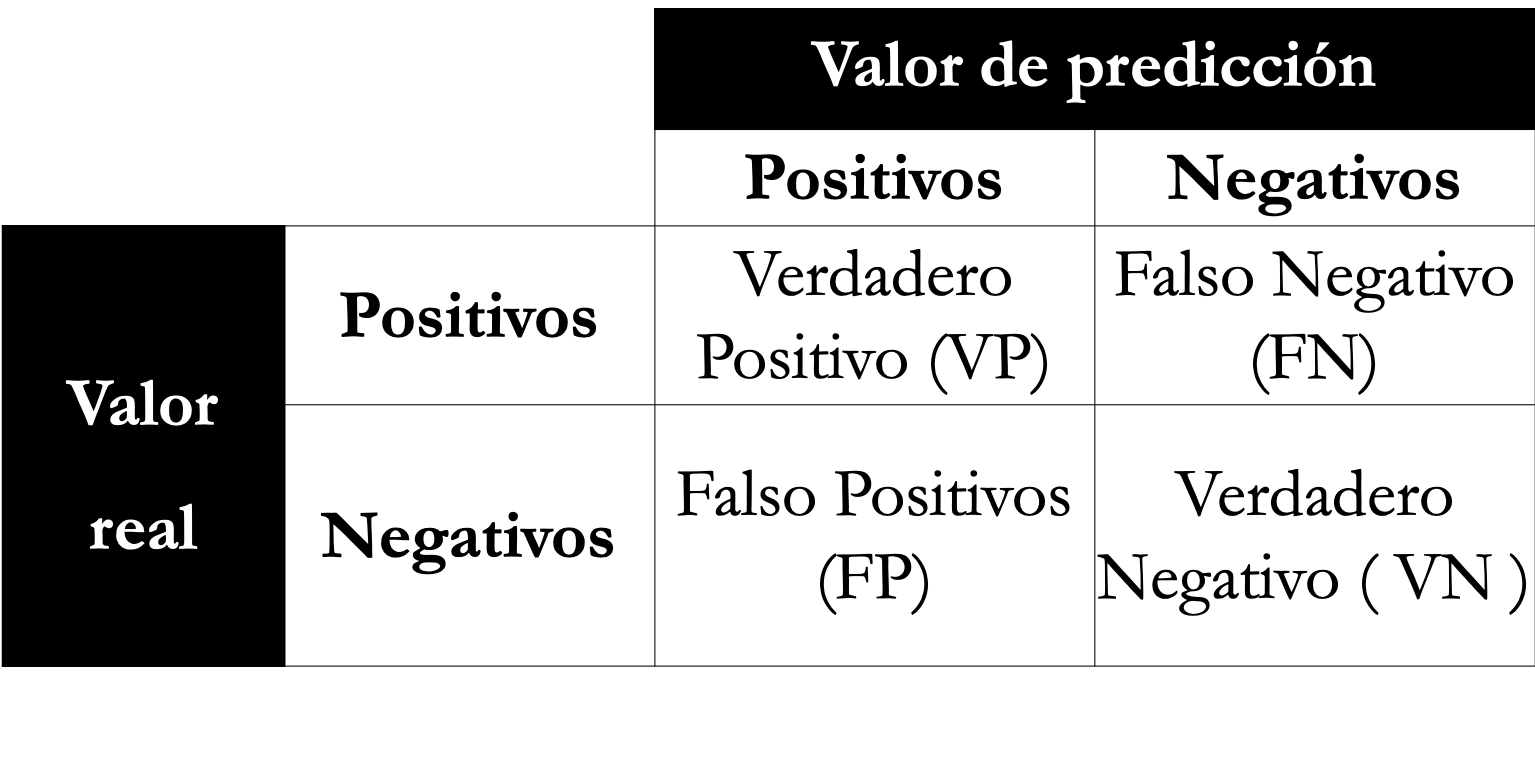
\includegraphics[scale=.4]{imagenes/Capitulo3/MatrizC.png}
	\caption{Matriz de confusión}
	\label{Fig:mconfu}
\end{figure}

La Figura \ref{Fig:mconfu} muestra un ejemplo de matriz de confusión con dos clases, la cual ejemplifica de
manera adecuada las diferentes entradas de la misma, entra las que se encuentran:


\begin{itemize}

	\item \textbf{VP}: Es la cantidad de datos positivos que fueron clasificados correctamente como positivos 
	\item \textbf{FN}: Es la cantidad de datos positivos que fueron clasificados incorrectamente como negativos
	\item \textbf{VN}: Es la cantidad de datos negativos que fueron clasificados correctamente como negativos
	\item \textbf{FP}: Es la cantidad de datos negativos que fueron clasificados incorrectamente como positivos
	
\end{itemize}

La diagonal principal en cualquier matriz de confusión n x n representa el número de predicciones
correctas para cada una de las n secciones.\\

Gracias a la matriz de confusión, es posible obtener ciertas métricas que nos ayudan a evaluar el modelo
de aprendizaje. Entre las que se encuentran:\\


\textbf{Exactitud}: es la proporción del número total de predicciones que son correctas respecto al total.
Se determina utilizando la ecuación:

\begin{equation}\label{eq:1}
	Exactitud = \frac{VP+VN}{VP+VN+FN+FP}
\end{equation}

\textbf{Recall}: Es la proporción de predicciones positivas que fueron correctamente clasificadas. Se determina
utilizando la ecuación:


\begin{equation}\label{eq:2}
	Recall = \frac{VP}{VP+FP}
\end{equation}


\textbf{Precisión}: Es la proporción de predicciones positivas que se clasificaron correctamente. Se determina
con la siguiente ecuación:


\begin{equation}\label{eq:3}
	Precision = \frac{VP}{VP+FN}
\end{equation}


\textbf{F-Measure (F1)}: Se interpreta como la media armónica entre Precisión y Recall. Se determina
con la siguiente ecuación:

\begin{equation}\label{eq:3}
	 F-Measure = 2 \cdot \frac{precision \cdot recall}{precision+recall}
\end{equation}

